
\documentclass{standalone}
\usepackage{amsmath, amsthm, amsfonts, amssymb}
\usepackage{tikz}
\usetikzlibrary{shapes,snakes,positioning,calc}

\newcommand{\disciplina}[6][nyellow]{
\node [draw=black, fill=#1, very thick, rectangle, rounded corners, inner
sep=2pt, inner ysep=2pt, text width=#5pt, minimum height=40pt,
text centered, anchor=west] (#4) at (#2,#3) {
   \begin{minipage}{#5pt}
   \linespread{1.0}\selectfont
       \centering
       \scriptsize{#6}
   \end{minipage}
};
}


\usepackage{xcolor}
\definecolor{nred}{rgb}{0.88, 0.28, 0.33}
\definecolor{nblue}{rgb}{0.34, 0.74, 0.96}
\definecolor{nyellow}{rgb}{0.8, 0.86, 0.38}
\definecolor{npurple}{rgb}{0.25, 0.34, 0.93}
\definecolor{ngreen}{rgb}{0.45, 0.95, 0.66}


\begin{document}

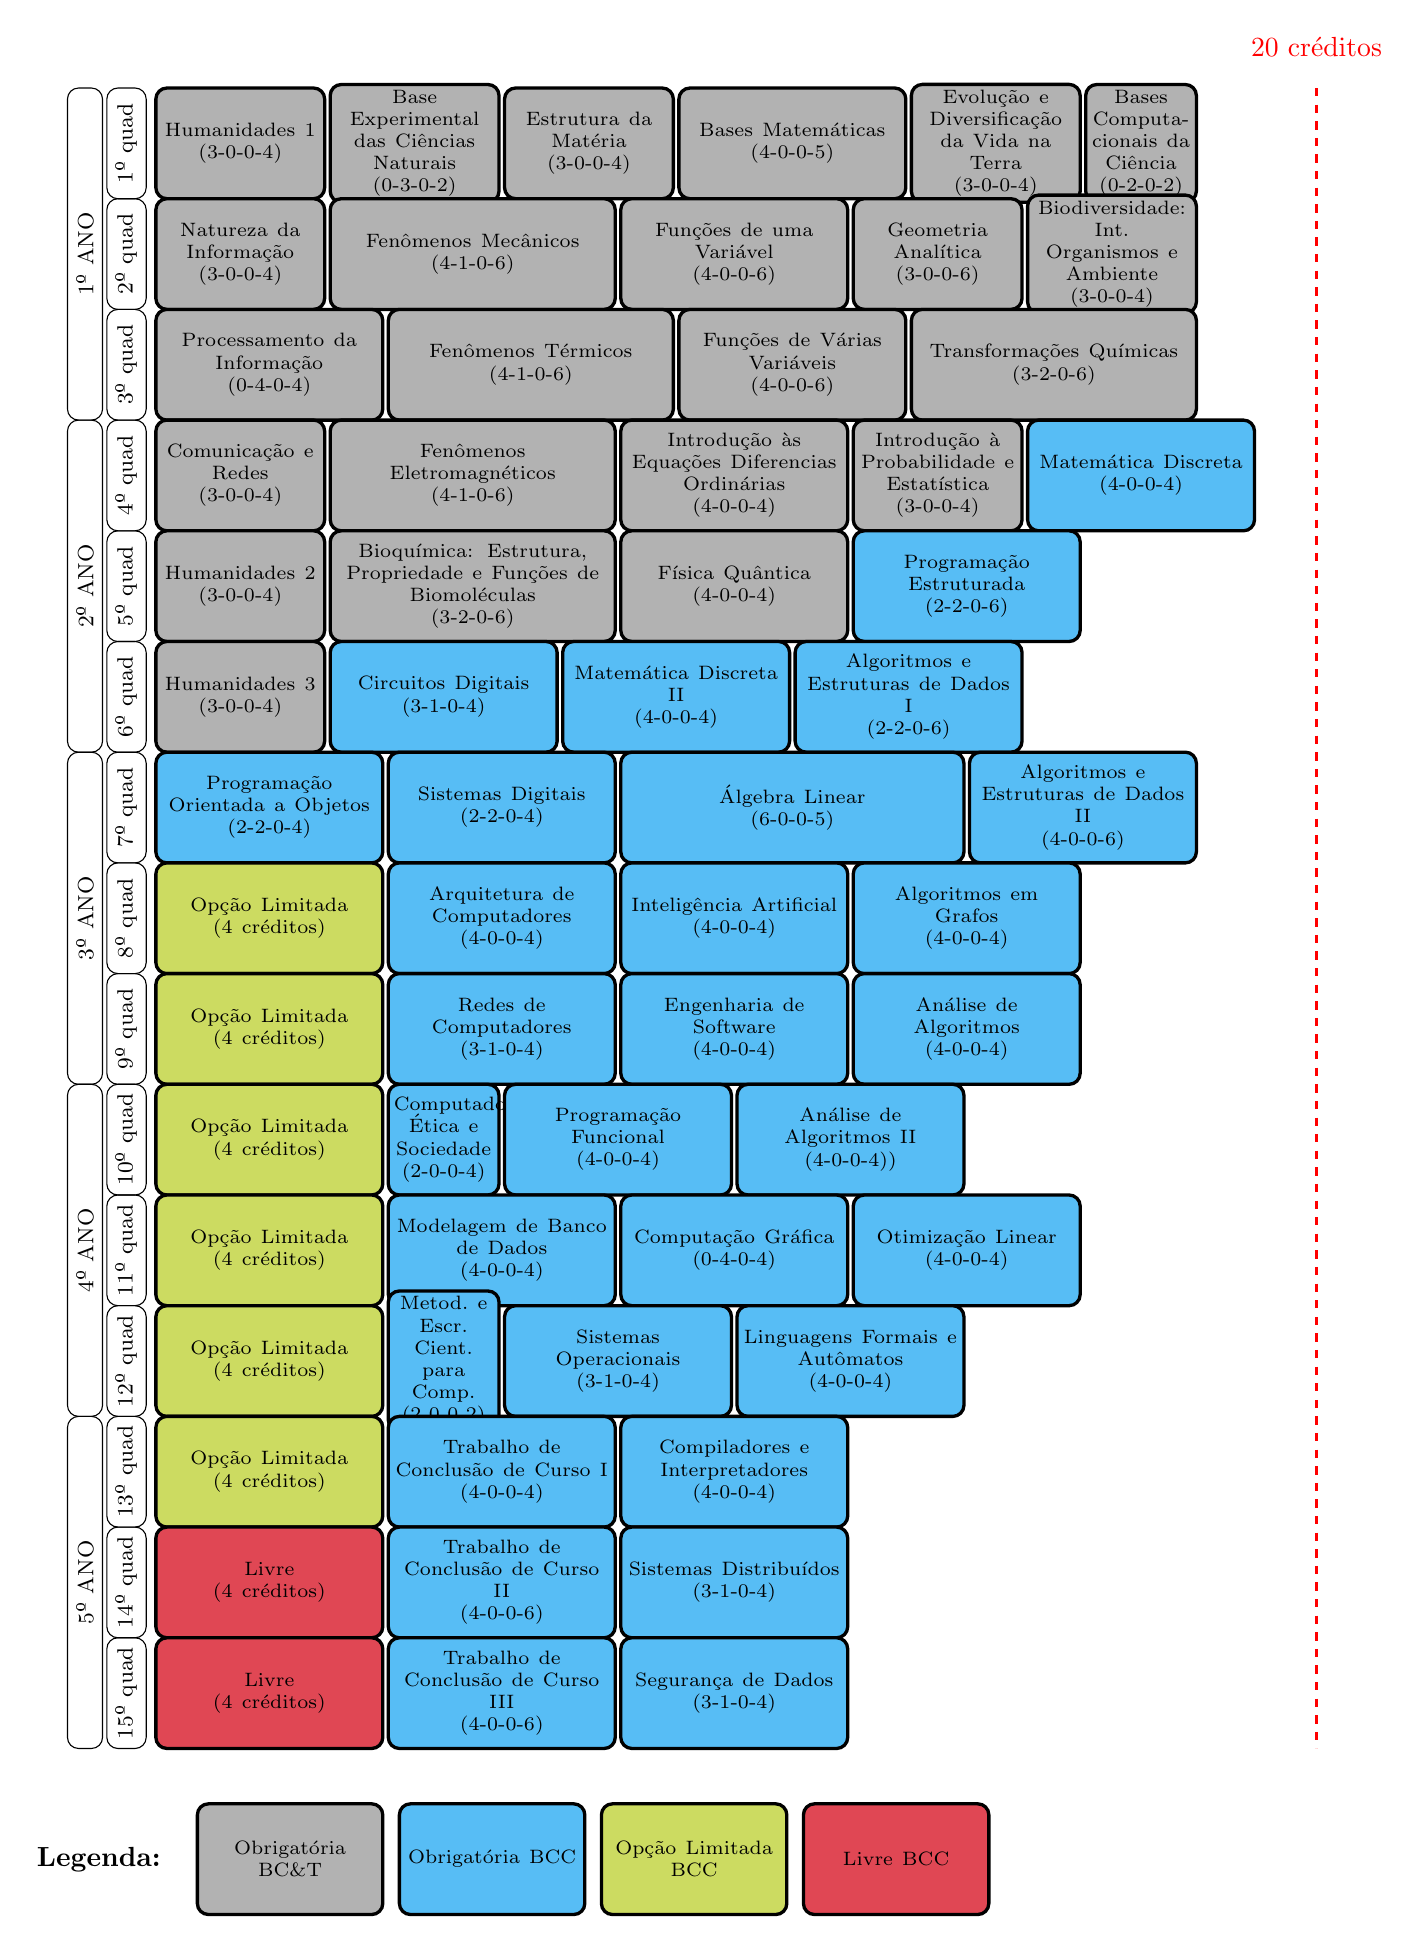
\begin{tikzpicture}

    \def\sz{21pt}
    \def\doisc{36} % 2*\sz - 6
    \def\tresc{57} % 3*\sz - 6
    \def\quatc{78} % 4*\sz - 6
    \def\cincc{99} % 5*\sz - 6
    \def\seisc{120} % 6*\sz - 6
    
    %Q1
    \node [draw, rotate=90, black,rectangle, minimum width=120pt, minimum
    height=10pt, rounded corners] at (-25pt,-40pt) {\footnotesize{1º ANO}};
    
    \node [draw, rotate=90, black,rectangle, minimum width=40pt, minimum
    height=10pt, rounded corners] at (-10pt,0pt) {\footnotesize{1º quad}};
    
    \disciplina [gray!60]{0*\sz}{0pt}{a}{\tresc}{Humanidades 1 \\(3-0-0-4)}
    
    \disciplina [gray!60]{3*\sz}{0pt}{b}{\tresc}{Base Experimental das Ciências Naturais\\ (0-3-0-2)} 
    
    \disciplina [gray!60]{6*\sz}{0pt}{c}{\tresc}{Estrutura da Matéria \\(3-0-0-4)}
    
    \disciplina [gray!60]{9*\sz}{0pt}{d}{\quatc}{Bases Matemáticas\\(4-0-0-5)}
    
    \disciplina [gray!60]{13*\sz}{0pt}{e}{\tresc}{Evolução e Diversificação da Vida na Terra \\(3-0-0-4)}
    
    \disciplina [gray!60]{16*\sz}{0pt}{f}{\doisc}{Bases Computacionais da Ciência \\(0-2-0-2)}
    
    
    %Q2
    \node [draw, rotate=90, black,rectangle, minimum width=40pt, minimum
    height=10pt, rounded corners] at (-10pt,-40pt) {\footnotesize{2º quad}};
    
    \disciplina [gray!60]{0*\sz}{-40pt}{a}{\tresc}{Natureza da Informação\\(3-0-0-4)}
    
    \disciplina [gray!60]{3*\sz}{-40pt}{a}{\cincc}{Fenômenos Mecânicos\\(4-1-0-6)}
    
    \disciplina [gray!60]{8*\sz}{-40pt}{a}{\quatc}{Funções de uma Variável\\(4-0-0-6)}
    
    \disciplina [gray!60]{12*\sz}{-40pt}{a}{\tresc}{Geometria Analítica\\(3-0-0-6)}
    
    \disciplina [gray!60]{15*\sz}{-40pt}{a}{\tresc}{Biodiversidade: Int. Organismos e Ambiente\\(3-0-0-4)}
    
    
    %Q3
    \node [draw, rotate=90, black,rectangle, minimum width=40pt, minimum
    height=10pt, rounded corners] at (-10pt,-80pt) {\footnotesize{3º quad}};
    
    \disciplina [gray!60]{0*\sz}{-80pt}{a}{\quatc}{Processamento da Informação\\(0-4-0-4)}
    
    \disciplina [gray!60]{4*\sz}{-80pt}{a}{\cincc}{Fenômenos Térmicos\\(4-1-0-6)}
    
    \disciplina [gray!60]{9*\sz}{-80pt}{a}{\quatc}{Funções de Várias Variáveis\\(4-0-0-6)}
    
    \disciplina [gray!60]{13*\sz}{-80pt}{a}{\cincc}{Transformações Químicas\\(3-2-0-6)}
    
    
    %Q4
    \node [draw, rotate=90, black,rectangle, minimum width=120pt, minimum
    height=10pt, rounded corners] at (-25pt,-160pt) {\footnotesize{2º ANO}};
    
    \node [draw, rotate=90, black,rectangle, minimum width=40pt, minimum
    height=10pt, rounded corners] at (-10pt,-120pt) {\footnotesize{4º quad}};
    
    \disciplina [gray!60]{0*\sz}{-120pt}{a}{\tresc}{Comunicação e Redes\\(3-0-0-4)}
    
    \disciplina [gray!60]{3*\sz}{-120pt}{a}{\cincc}{Fenômenos Eletromagnéticos\\(4-1-0-6)}
    
    \disciplina [gray!60]{8*\sz}{-120pt}{a}{\quatc}{Introdução às Equações Diferencias Ordinárias\\(4-0-0-4)}
    
    \disciplina [gray!60]{12*\sz}{-120pt}{a}{\tresc}{Introdução à Probabilidade e Estatística\\(3-0-0-4)}
    
    \disciplina [nblue]{15*\sz}{-120pt}{a}{\quatc}{Matemática Discreta\\(4-0-0-4)}

    
    %Q5
    \node [draw, rotate=90, black,rectangle, minimum width=40pt, minimum
    height=10pt, rounded corners] at (-10pt,-160pt) {\footnotesize{5º quad}};
    
    \disciplina [gray!60]{0*\sz}{-160pt}{a}{\tresc}{Humanidades 2\\(3-0-0-4)}
    
    \disciplina [gray!60]{3*\sz}{-160pt}{a}{\cincc}{Bioquímica: Estrutura, Propriedade e Funções de Biomoléculas\\(3-2-0-6)}
    
    \disciplina [gray!60]{8*\sz}{-160pt}{a}{\quatc}{Física Quântica\\(4-0-0-4)}
    
    \disciplina [nblue]{12*\sz}{-160pt}{a}{\quatc}{Programação Estruturada\\(2-2-0-6)}
    

    %Q6
    \node [draw, rotate=90, black,rectangle, minimum width=40pt, minimum
    height=10pt, rounded corners] at (-10pt,-200pt) {\footnotesize{6º quad}};
    
    \disciplina [gray!60]{0*\sz}{-200pt}{a}{\tresc}{Humanidades 3\\(3-0-0-4)}
    
    \disciplina [nblue]{3*\sz}{-200pt}{a}{\quatc}{Circuitos Digitais\\(3-1-0-4)}
    
    \disciplina [nblue]{7*\sz}{-200pt}{a}{\quatc}{Matemática Discreta II\\(4-0-0-4)}
    
    \disciplina [nblue]{11*\sz}{-200pt}{a}{\quatc}{Algoritmos e Estruturas de Dados I\\(2-2-0-6)}
    

    %Q7
    \node [draw, rotate=90, black,rectangle, minimum width=120pt, minimum
    height=10pt, rounded corners] at (-25pt,-280pt) {\footnotesize{3º ANO}};
    
    \node [draw, rotate=90, black,rectangle, minimum width=40pt, minimum
    height=10pt, rounded corners] at (-10pt,-240pt) {\footnotesize{7º quad}};
    
    \disciplina [nblue]{0*\sz}{-240pt}{a}{\quatc}{Programação Orientada a Objetos\\(2-2-0-4)}
    
    \disciplina [nblue]{4*\sz}{-240pt}{a}{\quatc}{Sistemas Digitais\\(2-2-0-4)}
    
    \disciplina [nblue]{8*\sz}{-240pt}{a}{\seisc}{Álgebra Linear\\(6-0-0-5)}
    
    \disciplina [nblue]{14*\sz}{-240pt}{a}{\quatc}{Algoritmos e Estruturas de Dados II\\(4-0-0-6)}
    
    
    %Q8
    \node [draw, rotate=90, black,rectangle, minimum width=40pt, minimum
    height=10pt, rounded corners] at (-10pt,-280pt) {\footnotesize{8º quad}};
    
    \disciplina [nyellow]{0*\sz}{-280pt}{a}{\quatc}{Opção Limitada\\(4 créditos)}
    
    \disciplina [nblue]{4*\sz}{-280pt}{a}{\quatc}{Arquitetura de Computadores\\(4-0-0-4)}
    
    \disciplina [nblue]{8*\sz}{-280pt}{a}{\quatc}{Inteligência Artificial\\(4-0-0-4)}
    
    \disciplina [nblue]{12*\sz}{-280pt}{a}{\quatc}{Algoritmos em Grafos\\(4-0-0-4)}
    
    
    %Q9
    \node [draw, rotate=90, black,rectangle, minimum width=40pt, minimum
    height=10pt, rounded corners] at (-10pt,-320pt) {\footnotesize{9º quad}};
    
    \disciplina [nyellow]{0*\sz}{-320pt}{a}{\quatc}{Opção Limitada\\(4 créditos)}
    
    \disciplina [nblue]{4*\sz}{-320pt}{a}{\quatc}{Redes de Computadores\\(3-1-0-4)}
    
    \disciplina [nblue]{8*\sz}{-320pt}{a}{\quatc}{Engenharia de Software\\(4-0-0-4)}
    
    \disciplina [nblue]{12*\sz}{-320pt}{a}{\quatc}{Análise de Algoritmos\\(4-0-0-4)}
    

    %Q10
    \node [draw, rotate=90, black,rectangle, minimum width=120pt, minimum
    height=10pt, rounded corners] at (-25pt,-400pt) {\footnotesize{4º ANO}};
    
    \node [draw, rotate=90, black,rectangle, minimum width=40pt, minimum
    height=10pt, rounded corners] at (-10pt,-360pt) {\footnotesize{10º quad}};
    
    \disciplina [nyellow]{0*\sz}{-360pt}{a}{\quatc}{Opção Limitada\\(4 créditos)}
    
    \disciplina [nblue]{4*\sz}{-360pt}{a}{\doisc}{Computadores, Ética e Sociedade\\(2-0-0-4)}
    
    \disciplina [nblue]{6*\sz}{-360pt}{a}{\quatc}{Programação Funcional\\(4-0-0-4)}
    
    \disciplina [nblue]{10*\sz}{-360pt}{a}{\quatc}{Análise de Algoritmos II\\(4-0-0-4))}
    
    
    %Q11
    \node [draw, rotate=90, black,rectangle, minimum width=40pt, minimum
    height=10pt, rounded corners] at (-10pt,-400pt) {\footnotesize{11º quad}};
    
    \disciplina [nyellow]{0*\sz}{-400pt}{a}{\quatc}{Opção Limitada\\(4 créditos)}
    
    \disciplina [nblue]{4*\sz}{-400pt}{a}{\quatc}{Modelagem de Banco de Dados\\(4-0-0-4)}
    
    \disciplina [nblue]{8*\sz}{-400pt}{a}{\quatc}{Computação Gráfica\\(0-4-0-4)}
    
    \disciplina [nblue]{12*\sz}{-400pt}{a}{\quatc}{Otimização Linear\\(4-0-0-4)}
    
    %Q12
    \node [draw, rotate=90, black,rectangle, minimum width=40pt, minimum
    height=10pt, rounded corners] at (-10pt,-440pt) {\footnotesize{12º quad}};
    
    \disciplina [nyellow]{0*\sz}{-440pt}{a}{\quatc}{Opção Limitada\\(4 créditos)}
    
    \disciplina [nblue]{4*\sz}{-440pt}{a}{\doisc}{Metod.\ e Escr.\ Cient.\ para Comp.\\(2-0-0-2)}
    
    \disciplina [nblue]{6*\sz}{-440pt}{a}{\quatc}{Sistemas Operacionais\\(3-1-0-4)}
    
    \disciplina [nblue]{10*\sz}{-440pt}{a}{\quatc}{Linguagens Formais e Autômatos\\(4-0-0-4)}
    

    %Q13
    \node [draw, rotate=90, black,rectangle, minimum width=120pt, minimum
    height=10pt, rounded corners] at (-25pt,-520pt) {\footnotesize{5º ANO}};
    
    \node [draw, rotate=90, black,rectangle, minimum width=40pt, minimum
    height=10pt, rounded corners] at (-10pt,-480pt) {\footnotesize{13º quad}};
    
    \disciplina [nyellow]{0*\sz}{-480pt}{a}{\quatc}{Opção Limitada\\(4 créditos)}
    
    \disciplina [nblue]{4*\sz}{-480pt}{a}{\quatc}{Trabalho de Conclusão de Curso I\\(4-0-0-4)}
    
    \disciplina [nblue]{8*\sz}{-480pt}{a}{\quatc}{Compiladores e Interpretadores\\(4-0-0-4)}
    
    
    %Q14
    \node [draw, rotate=90, black,rectangle, minimum width=40pt, minimum
    height=10pt, rounded corners] at (-10pt,-520pt) {\footnotesize{14º quad}};
    
    \disciplina [nred]{0*\sz}{-520pt}{a}{\quatc}{Livre\\(4 créditos)}
    
    \disciplina [nblue]{4*\sz}{-520pt}{a}{\quatc}{Trabalho de Conclusão de Curso II\\(4-0-0-6)}
    
    \disciplina [nblue]{8*\sz}{-520pt}{a}{\quatc}{Sistemas Distribuídos\\(3-1-0-4)}
    

    %Q15
    \node [draw, rotate=90, black,rectangle, minimum width=40pt, minimum
    height=10pt, rounded corners] at (-10pt,-560pt) {\footnotesize{15º quad}};
    
    \disciplina [nred]{0*\sz}{-560pt}{a}{\quatc}{Livre\\(4 créditos)}

    \disciplina [nblue]{4*\sz}{-560pt}{a}{\quatc}{Trabalho de Conclusão de Curso III\\(4-0-0-6)}
    
    \disciplina [nblue]{8*\sz}{-560pt}{a}{\quatc}{Segurança de Dados\\(3-1-0-4)}
    
    
    \draw [red,thick,dashed] (20*\sz,20pt) -- (20*\sz,-580pt); 
    \node [text=red] at (420pt,35pt) {20 créditos};


    \node [text=black] at (-20pt, -620pt) {\textbf{Legenda:} }	;
    \disciplina [gray!60]{15pt}{-620pt}{bis0505}{63}{Obrigatória BC\&T}
    
    \disciplina [nblue]{88pt}{-620pt}{bis0505}{63}{Obrigatória BCC}
    
    \disciplina [nyellow]{161pt}{-620pt}{bis0505}{63}{Opção Limitada BCC}
    
    \disciplina [nred]{234pt}{-620pt}{bis0505}{63}{Livre BCC}
    
    
\end{tikzpicture}


\end{document}
